
%% ``particle shape analysis''
\section{Análise de partículas ou cúmulos}
\label{sec:cumulos}
Dada uma matriz binária $\MATRIX{M}\in \mathbb{B}^{N_l \times N_c}$, 
que representa uma imagem  em branco e preto, como é mostrado na
Eq. (\ref{eq:matrixM}) e na Figura \ref{fig:motivacion-M}, 
onde os pixels de cor branca tem valor $1$ e as de cor preta valor $0$. 
Podemos representar $\MATRIX{M}$ como a agrupação de um conjunto de vetores coluna
$\MATRIX{M}=[\VECTOR{m}_1\quad\VECTOR{m}_2\quad...\quad\VECTOR{m}_c\quad...\quad\VECTOR{m}_{N_c}]$,
por outro lado podemos representar a um elemento da matriz $\MATRIX{M}$ como
$\MATRIX{M}(l,c)$, onde $l$ e $c$ representam a posição da linha e coluna respetivamente.
\setcounter{MaxMatrixCols}{25}
\begin{equation}\label{eq:matrixM}
\MATRIX{M}=
\begin{bmatrix}
1 & 0 & 0 & 1 & 1 & 0 & 0 & 0 & 0 & 1 & 0 & 0 \\ 
0 & 0 & 0 & 0 & 0 & 0 & 0 & 0 & 0 & 0 & 0 & 0 \\
0 & 0 & 1 & 1 & 1 & 1 & 1 & 1 & 1 & 1 & 1 & 1 \\
0 & 1 & 1 & 0 & 0 & 0 & 0 & 0 & 1 & 0 & 0 & 0 \\
1 & 1 & 0 & 0 & 0 & 0 & 0 & 1 & 1 & 1 & 0 & 0 \\ 
1 & 0 & 0 & 0 & 1 & 1 & 1 & 1 & 0 & 1 & 1 & 1 \\
0 & 0 & 1 & 0 & 0 & 0 & 0 & 0 & 0 & 0 & 0 & 0 \\
0 & 1 & 1 & 0 & 0 & 0 & 1 & 1 & 0 & 0 & 1 & 1 
\end{bmatrix}
\end{equation}
\begin{figure}[!h]
\centering
    \begin{subfigure}[t]{0.4\textwidth}
        \centering
        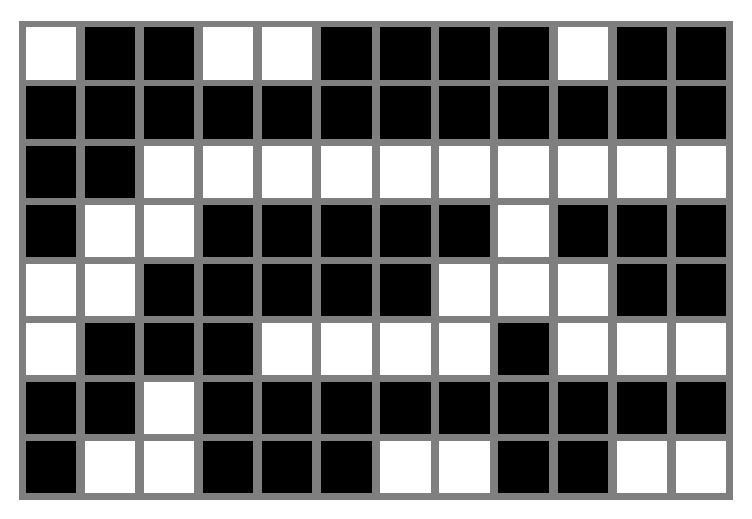
\includegraphics[width=\textwidth]{section-cumulos/motivacion-M.eps}
        \caption{Matriz binária $\MATRIX{M}$ representada como uma imagem em branco e preto.}
        \label{fig:motivacion-M}
    \end{subfigure}%
    \hfill%
    \begin{subfigure}[t]{0.4\textwidth}
        \centering
        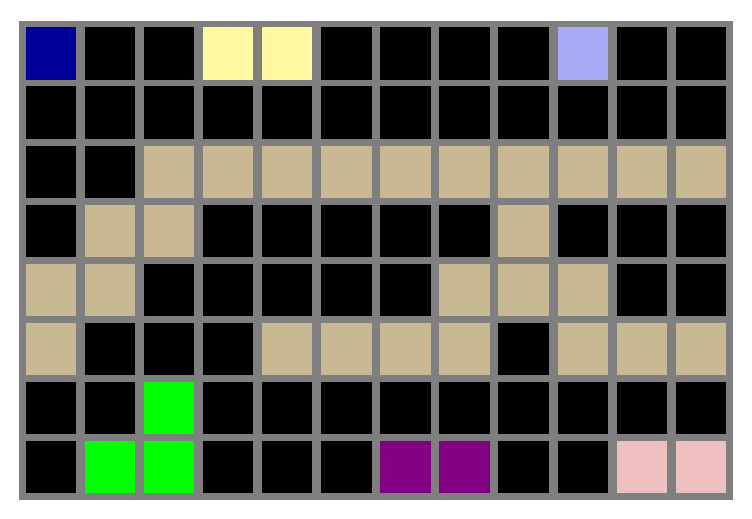
\includegraphics[width=\textwidth]{section-cumulos/motivacion-GMAP.eps}
        \caption{Matriz $\MATRIX{G}$ com valores inteiros, 
        representada como uma imagem com partículas (cúmulos) formados por grupos de pixels brancos.}
        \label{fig:motivacion-G}
    \end{subfigure}
\caption{Analisando partículas na matriz $\MATRIX{M}$.}
\label{fig:motivacion}
\end{figure}


A Figura \ref{fig:Diagrama} mostra um diagrama de bloco de um detetor de cúmulos,
o bloco recebe como entrada uma matriz binária $\MATRIX{M}$ e 
retorna uma matriz inteira $\MATRIX{G}\in \mathbb{N}^{N_l \times N_c}$, 
criada pela agrupação dos pixels brancos em cúmulos, como na Figura \ref{fig:motivacion-G}; onde 
todos os pixels num cúmulo são mapeados com o mesmo índice\footnote{Na 
figura cada diferente $id$ está representado com uma diferente cor.} 
$id$. % $\forall~0 \leq id \leq L$.
O identificador $id=0$ corresponde aos pixels pretos, é dizer os bits 0,
qualquer outro $id$ tomará um valor maior a zero.

\begin{figure}[!htb]
\centering
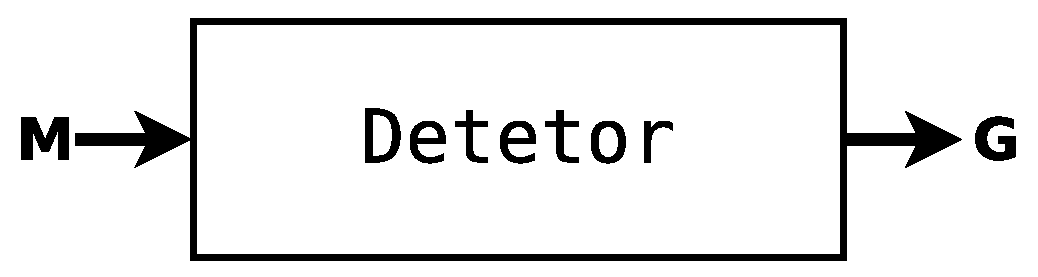
\includegraphics[width=0.35\textwidth]{section-cumulos/Diagrama.eps}
\caption{Diagrama de bloco do sistema.}
\label{fig:Diagrama}
\end{figure}



%%%%%%%%%%%%%%%%%%%%%%%%%%%%%%%%%%%%%%%%%%%%%%%%%%%%%%%%%%%%%%%%%%%%%%%%%%%%%%%%
\subsection{Detetor de cúmulos}
\label{subsec:part1}

Nosso problema principal é obter, a partir de uma matriz $\MATRIX{M}$, 
 uma matriz $\MATRIX{G}$ onde cada elemento contem
o índice do cúmulo ao qual pertence, como mostra a Figura \ref{fig:motivacion}.
Assim, pra cumprir este objetivo são usadas as funções $funA$ e $funB$, como mostra  a
Figura \ref{fig:modelocumulos}, onde são analisadas de maneira sequencial as colunas $\VECTOR{M}_c$ da
matriz $\MATRIX{M}$.
\begin{figure}[!htb]
\centering
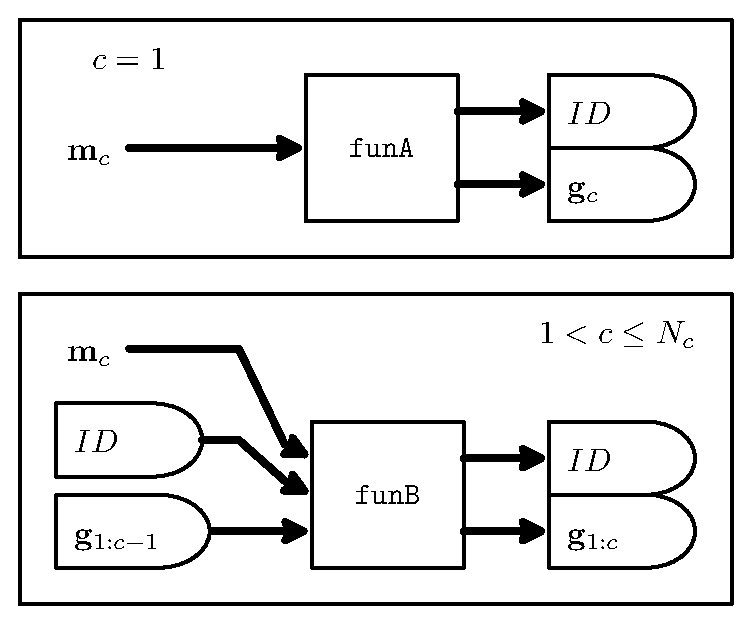
\includegraphics[width=0.45\textwidth]{section-cumulos/DiagramaCompleto.eps}
\caption{Diagrama de fluxo del algoritmo de criação de cúmulos.}
\label{fig:modelocumulos}
\end{figure}

\begin{itemize}
\item A função $funA$ recebe como parâmetro de entrada a coluna $\VECTOR{m}_1$ $\in\MATRIX{M}$.
Retorna o valor dos índices na coluna $\VECTOR{g}_1$ $\in\MATRIX{G}$;
adicionalmente a função retorna, $ID$, 
o valor do maior identificador $id$ atribuído aos cúmulos nas operações.

\item A função $funB$ recebe como parâmetros de entrada a $c$-ésima 
coluna $\VECTOR{m}_c$ $\in\MATRIX{M}$, o mapa de índices na submatriz $\VECTOR{g}_{1:(c-1)}$ $\in\MATRIX{G}$
que abrange informações de índice desde a primeira coluna ate a $(c-1)$-ésima e
$ID$ o valor do maior identificador $id$ atribuído aos cúmulos nas operações.
A função retorna a matriz $\VECTOR{g}_{1:c}$ com os dados dos índices desde a primeira coluna ate a $c$-ésima,
adicionalmente a função retorna o novo valor de $ID$.
\end{itemize}

%%%%%%%%%%%%%%%%%%%%%%%%%%%%%%%%%%%%%%%%%%%%%%%%%%%%%%%%%%%%%%%%%%%%%%%%%%%%%%%%
\subsubsection{Algoritmo da função $funA$}
\label{subsubsec:funA}
A função $funA$ recebe um vetor coluna $\VECTOR{m}_1$ com uns e zeros, como é exemplificado na
Figura \ref{fig:funA}, na saída a função retorna um vetor $\VECTOR{g}_1$ com o mesmo tamanho
porem com elementos com valores inteiros; este vetor representa o mapeamento dos índices $id$ em cada cumulo de $\VECTOR{m}_1$.
\begin{figure}[!htb]
\centering
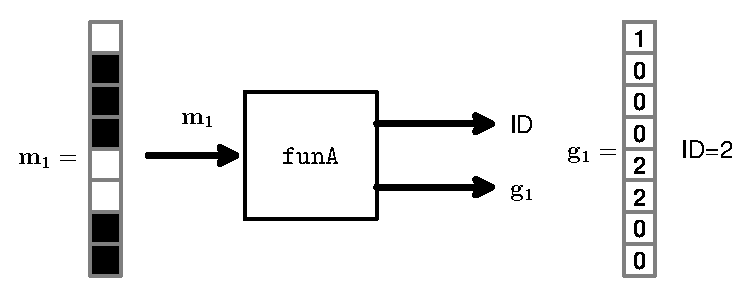
\includegraphics[width=0.7\textwidth]{section-cumulos/funA.eps}
\caption{Descrição da função $funA$.}
\label{fig:funA}
\end{figure}

Para calcular $\VECTOR{g}_1$ se usa o vetor $\VECTOR{m}_1$;
elementos com zero em $\VECTOR{m}_1$ provocam automaticamente elementos com um índice $0$ em $\VECTOR{g}_1$;
por outro lado, se achamos uma região de $1$'s em $\VECTOR{m}_1$, 
estes recebem em $\VECTOR{g}_1$ um mesmo índice,
sendo que cada região de $1$'s tem um índice diferente. 
A função $funA$ também retorna, $ID$, o máximo índice estabelecido em $\VECTOR{g}_1$.
Um algoritmo que explica este procedimento, pode ser visto no diagrama de fluxo da Figura \ref{fig:funA0};
o algoritmo usa a função $funB1$ copia zeros do vetor $\VECTOR{m}_1$ ao vetor $\VECTOR{g}_1$;
mais detalhes da função são explicados na Seção \ref{subsubsec:funB}.
\begin{figure}[!htb]
\centering
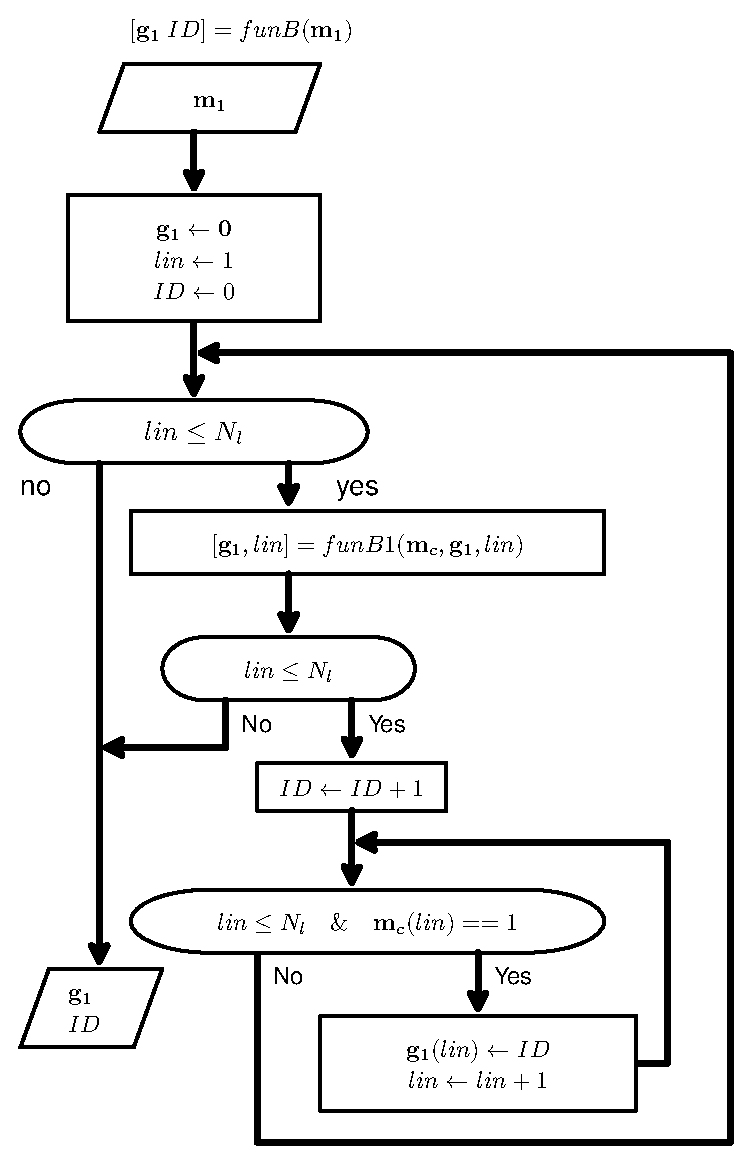
\includegraphics[width=0.5\textwidth]{section-cumulos/funA0.eps}
\caption{Descrição da função $funA$.}
\label{fig:funA0}
\end{figure}

%%%%%%%%%%%%%%%%%%%%%%%%%%%%%%%%%%%%%%%%%%%%%%%%%%%%%%%%%%%%%%%%%%%%%%%%%%%%%%%%
\subsubsection{Algoritmo da função $funB$}
\label{subsubsec:funB}
A função $funB$ recebe como parâmetros de entrada um vetor $\VECTOR{m}_{c}$, correspondente a 
$c$-ésima coluna da matriz $\MATRIX{M}$, a submatriz $\VECTOR{g}_{1:(c-1)}$ $\in\MATRIX{G}$ com o mapa de índices
desde a primeira coluna ate a $(c-1)$-ésima coluna da matriz $\MATRIX{G}$, 
e o máximo índice $ID$ nos elementos da matriz $\VECTOR{g}_{1:(c-1)}$. 
Na saída a função retorna uma matriz $\VECTOR{g}_{1:c}$ $\in\MATRIX{G}$ com o mapa de grupos
desde a primeira coluna ate a $c$-ésima coluna da matriz $\MATRIX{G}$, 
e o máximo índice $ID$ achado na matriz $\VECTOR{g}_{1:c}$.
A Figura \ref{fig:funB} mostra o diagrama fluxo do algoritmo da função $funB$.
\begin{figure}[!htb]
\centering
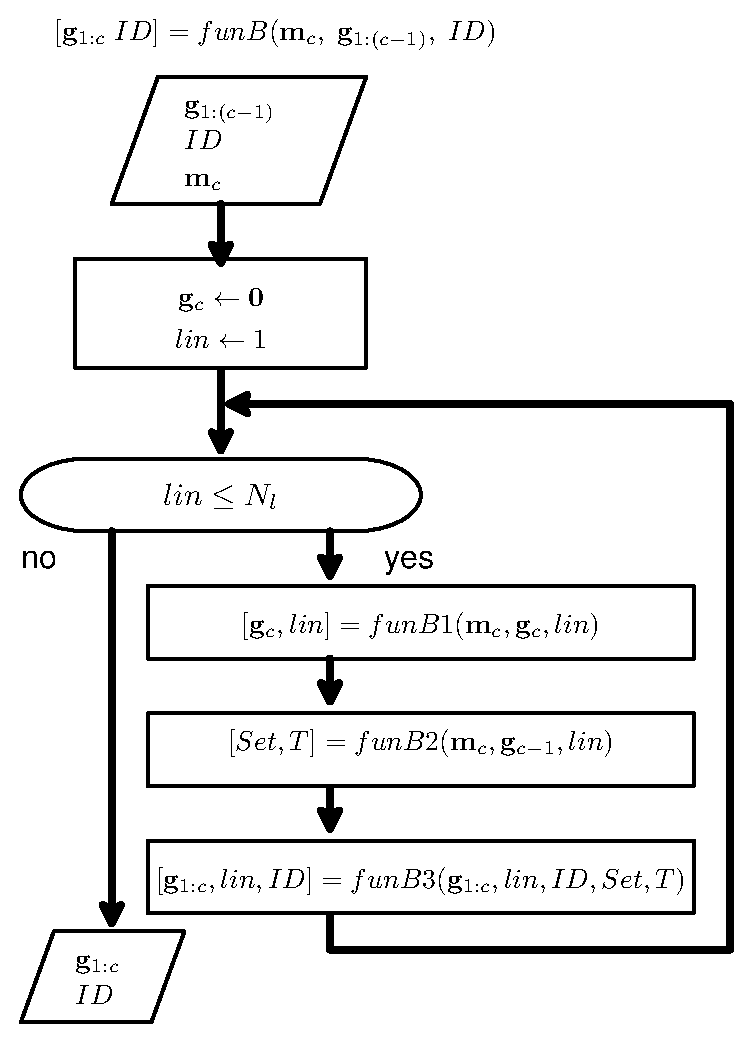
\includegraphics[width=0.45\textwidth]{section-cumulos/funB.eps}
\caption{Descrição da função $funB$ }
\label{fig:funB}
\end{figure}
A função $funB$ analisa os elementos do vetor $\VECTOR{m}_{c}$, desde o primeiro
elemento ate o elemento $N_l$; isto é realizado mediante as funções auxiliares $funB1$, $funB2$ e $funB3$,
de modo que estas funções modificam o conteúdo da matriz $\VECTOR{g}_{1:c}$ e a variável $ID$.

\textbf{Algoritmo da função $funB1$}:
A função recebe como parâmetros de entrada os vetores $\VECTOR{m}_{c}$, $\VECTOR{g}_{c}$
e uma variável com a linha $lin$ onde inciara o analises.
Se existem zeros no vetor $\VECTOR{m}_{c}$, então se escrevem zeros nos elementos na mesma posição 
no vetor $\VECTOR{g}_{c}$.
A função finaliza quando se acha o primeiro $1$ no vetor $\VECTOR{m}_{c}$,
carregando esta posição na variável $lin$, 
como mostra o diagrama de fluxo da Figura \ref{fig:funB1}.
\begin{figure}[!htb]
\centering
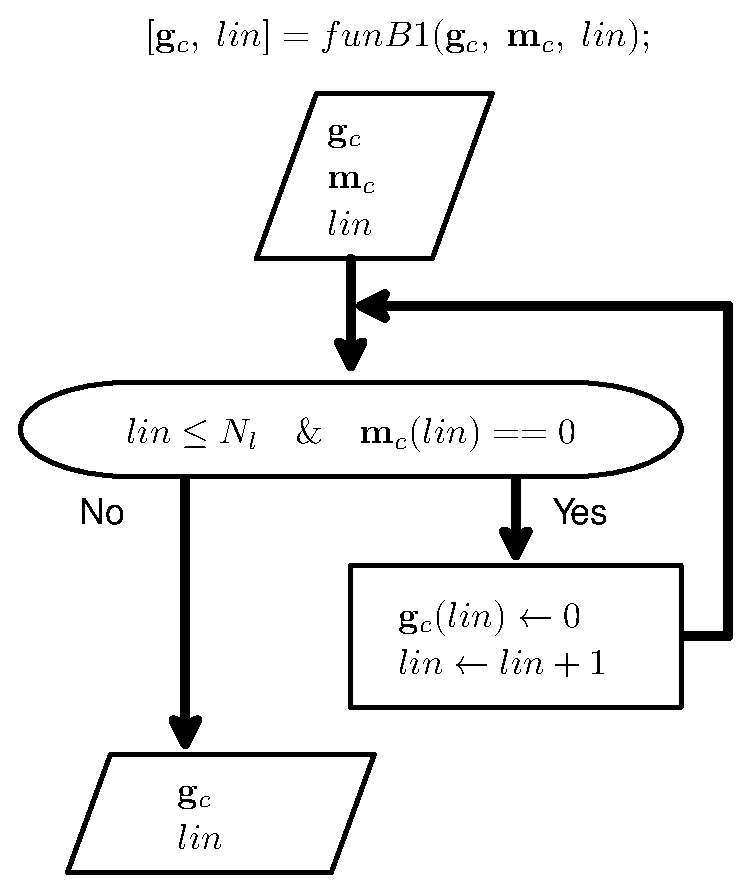
\includegraphics[width=0.45\textwidth]{section-cumulos/funB1.eps}
\caption{Descrição da função $funB1$ }
\label{fig:funB1}
\end{figure}

\textbf{Algoritmo da função $funB2$}:
A função recebe como parâmetros de entrada os vetores $\VECTOR{m}_{c}$, $\VECTOR{g}_{c-1}$
e uma variável com a linha $lin$ que indica a posição do primeiro $1$ achado com a função $funB1$. 
A função $funB2$ analisa somente um cumulo de $1$'s no vetor $\VECTOR{m}_{c}$, 
retornando um conjunto, $Set$, com os $id$'s no $\VECTOR{g}_{c-1}$ 
que estejam ao lado dos uns analisados no cúmulo em $\VECTOR{m}_{c}$;
adicionalmente a função $funB2$ retorna, $T$, o número de $1$'s do cúmulo.
O algoritmo da função $funB2$ pode ser visto no diagrama de fluxo da Figura \ref{fig:funB2};
nele podemos perceber o uso da função $Set.AddNoZero(id)$,
esta função agrega o índice $id$ ao conjunto $Set$,
se este ainda não existe em $Set$ e se $id\neq 0$.
\begin{figure}[!htb]
\centering
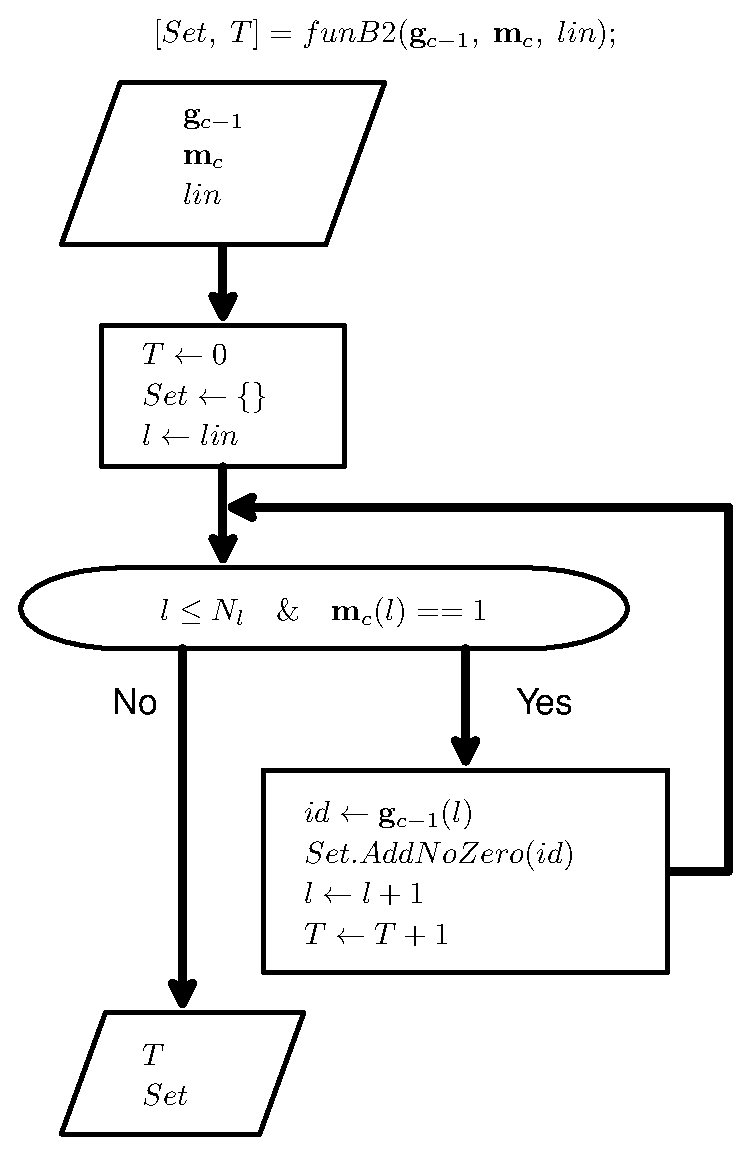
\includegraphics[width=0.45\textwidth]{section-cumulos/funB2.eps}
\caption{Descrição da função $funB2$ }
\label{fig:funB2}
\end{figure}

\textbf{Algoritmo da função $funB3$}:
A função recebe como parâmetros de entrada a submatriz $\VECTOR{g}_{1:c}$ $\in\MATRIX{G}$, 
uma variável com a linha $lin$ que indica a posição do primeiro $1$ achado com a função $funB1$,
o índice $ID$ que contem o valor do máximo $id$ nos elementos da submatriz $\VECTOR{g}_{1:(c-1)}$ $\in\MATRIX{G}$,
um conjunto $Set$ com todos os índice vizinhos ao cúmulo analisado com a função $funB2$,
e finalmente, $T$, o número de $1$'s no cúmulo.
A função $funB3$ se encarrega de escrever no vetor $\VECTOR{g}_{c}$ o índice correspondente,
e fusionar índices na submatriz $\VECTOR{g}_{1:(c-1)}$ se for necessário;
assim, a função retorna a submatriz $\VECTOR{g}_{1:c}$, com os índices modificados ate a $c$-ésima coluna 
e $lin$-ésima linha, também retorna o atual valor de $lin$ que indica o lugar do primeiro $0$ achado,
finalmente a função retorna o índice, $ID$, com maior valor achado na submatriz  $\VECTOR{g}_{1:c}$.
O algoritmo da função $funB3$ pode ser visto no diagrama de fluxo da Figura \ref{fig:funB3};
nele podemos perceber o uso da função $funC$,
esta função troca todos os índices $id$ em $\VECTOR{g}_{1:c-1}$, que existam no conjunto $Set$,
pelo valor do primeiro índice no conjunto $Set$, de modo que todo os elementos achados em 
$\VECTOR{g}_{1:c-1}$ tenham o índice $Set.at(1)$.
\begin{figure}[!htb]
\centering
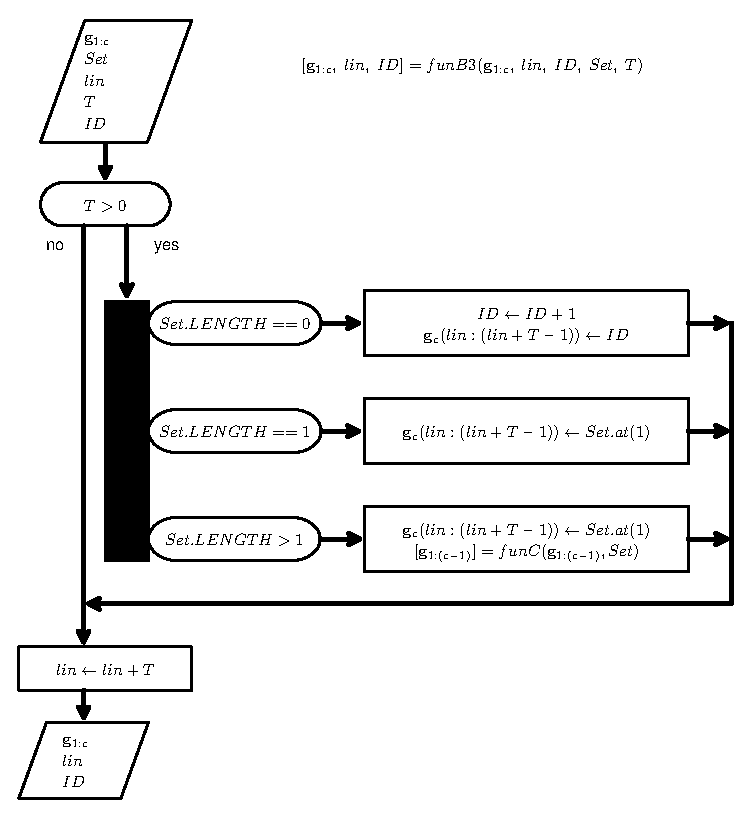
\includegraphics[width=0.65\textwidth]{section-cumulos/funB3.eps}
\caption{Descrição da função $funB3$ }
\label{fig:funB3}
\end{figure}

%%%%%%%%%%%%%%%%%%%%%%%%%%%%%%%%%%%%%%%%%%%%%%%%%%%%%%%%%%%%%%%%%%%%%%%%%%%%%%%%
%%%%%%%%%%%%%%%%%%%%%%%%%%%%%%%%%%%%%%%%%%%%%%%%%%%%%%%%%%%%%%%%%%%%%%%%%%%%%%%%
\subsection{Estatística da matriz $\MATRIX{G}$ }
\label{subsec:part1}


A informação em $\MATRIX{G}$ pode ser processada para 
retornar uma vetor $\VECTOR{s}$ com $L$ elementos, um por cada cúmulo,
onde $\VECTOR{s}(l)$ representa ao $l$-ésimo cúmulo analisado,
ver Figura \ref{fig:Diagrama2}.
Assim $\VECTOR{s}$ é uma estrutura que contem 
dados e estatística de cada cúmulo como:
\begin{itemize}
%\item Uma lista de todos os pixels no cúmulo com um identificador $id$.
\item $\VECTOR{s}(l).Id$ : O índice atribuído ao $l$-ésimo cúmulo.
\item $\VECTOR{s}(l).Area$ : A área em pixels do $l$-ésimo cúmulo.
%\item Centroide.
\end{itemize}


\begin{figure}[!htb]
\centering
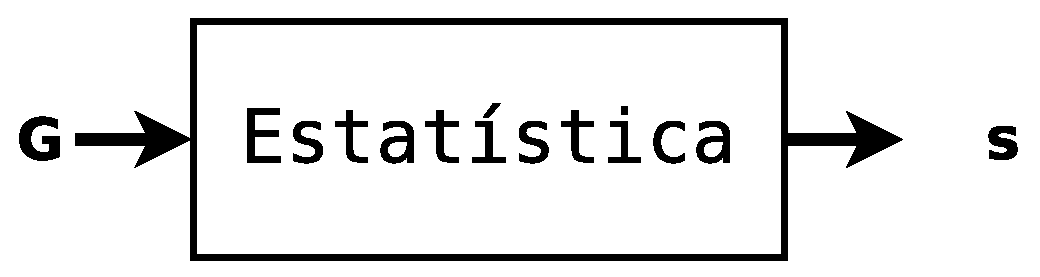
\includegraphics[width=0.35\textwidth]{section-cumulos/Diagrama2.eps}
\caption{Diagrama de bloco para obter estatística de $\MATRIX{G}$.}
\label{fig:Diagrama2}
\end{figure}

